\documentclass[10pt,letterpaper]{article}
\usepackage[utf8]{inputenc}
\usepackage[spanish,es-nodecimaldot]{babel}
\usepackage[margin=2.0cm,top=2.2cm,bottom=2.2cm]{geometry}
\usepackage{amsmath,amssymb,amsfonts}
\usepackage{booktabs}
\usepackage{graphicx}
\graphicspath{{../outputs/}{outputs/}}
\usepackage{hyperref}
\usepackage{fancyhdr}
\usepackage{microtype}
\usepackage{caption}
\usepackage{float}
\usepackage{parskip}

% Hipervínculos sobrios
\hypersetup{
    colorlinks=true,
    linkcolor=black,
    citecolor=black,
    urlcolor=blue!70!black
}

% Encabezado y pie de página limpios y académicos
\pagestyle{fancy}
\fancyhf{}
\fancyhead[L]{\small \textit{CC2017 Modelación y Simulación — Examen Práctico}}
\fancyhead[R]{\small \textit{Grupo 1: Población Desplazada}}
\fancyfoot[C]{\thepage}
\renewcommand{\headrulewidth}{0.4pt}
\renewcommand{\footrulewidth}{0pt}

\begin{document}

% Portada / Encabezado sobrio y natural
\begin{center}
    {\large Universidad del Valle de Guatemala}\\[2pt]
    {\normalsize Facultad de Ingeniería — Departamento de Ciencias de la Computación}\\[2pt]
    {\small CC2017: Modelación y Simulación — Ciclo 2026}\\[16pt]
    
    {\Large\textbf{Dinámica de Población Desplazada y Capacidad de Albergues}}\\[4pt]
    {\large Análisis de Saturación, Habitabilidad de Viviendas y Simulación post-Terremoto en Ciudad UVG}\\[12pt]
    
    \textbf{Unidad Técnica — Grupo 1}\\[4pt]
    \small 8 de septiembre de 2026
\end{center}

\vspace{10pt}
\hrule
\vspace{15pt}

% ==============================================================================
% SECCIÓN 1: JUSTIFICACIÓN DEL PARADIGMA
% ==============================================================================
\section{Justificación del paradigma de simulación}

Para modelar la respuesta de la ciudad tras el terremoto de magnitud 6.8, nuestro grupo eligió el paradigma de \textbf{Dinámica de Sistemas (System Dynamics, SD)}, implementado en tiempo discreto con bloques de 6 horas durante un horizonte de 72 horas. 

Esta decisión responde directamente al nivel de detalle y al tipo de preguntas que la Municipalidad y el Comité de Emergencia necesitan resolver. Nuestro objetivo principal es proyectar balances poblacionales agregados por zona urbana: cuántas personas necesitan refugio en cada momento, a qué velocidad se llenan los albergues y cuántas personas quedan sin atención en la vía pública. Para responder esto de forma confiable, no es necesario conocer las características individuales ni las historias de vida de los 250,000 habitantes de la ciudad; lo que determina el comportamiento del sistema son los flujos masivos de personas y los cuellos de botella generados por la capacidad finita de las instalaciones.

La dinámica de ocupación de albergues encaja de forma natural en la estructura de \textit{stocks} y flujos de la Dinámica de Sistemas. Cada albergue funciona como un acumulador con un límite físico bien definido. Mientras exista espacio disponible, las personas que van llegando son admitidas; una vez que el albergue se llena, el flujo de entrada a las instalaciones cae a cero y los damnificados que siguen llegando se desvían necesariamente a un segundo stock acumulador: la población sin alojamiento en espacios públicos. Esta regla de saturación no lineal, gobernada por restricciones físicas de capacidad, se modela de manera exacta y transparente mediante ecuaciones de balance.

\subsection{Frontera con los paradigmas de los otros grupos}
En la cadena de coordinación de la emergencia, cada unidad técnica trabaja con el paradigma que mejor se adapta a su problema:

\begin{itemize}
    \item \textbf{Conexión con Grupo 6 (Comportamiento poblacional):} El Grupo 6 modela las decisiones individuales de las familias (el miedo a réplicas, la desinformación en redes sociales o la incapacidad física de autoevacuar). Esas conductas heterogéneas requieren Modelado Basado en Agentes (ABM). Sin embargo, el Grupo 1 no necesita replicar esos agentes en su modelo: el Grupo 6 procesa esas decisiones y nos entrega el resultado final resumido, que es la proyección del flujo de evacuación por zona a lo largo del tiempo. Nosotros tomamos ese dato como una tasa de entrada y calculamos cómo impacta en los albergues.
    \item \textbf{Conexión con Grupos 2 y 3 (Hospitales y Suministros):} Los sistemas hospitalarios y las cadenas de distribución suelen modelarse mediante Simulación de Eventos Discretos (DES), porque dependen de colas de espera en triage, tiempos de atención médica o salidas programadas de convoys. Nuestro modelo en SD calcula la demanda agregada esperada (el 18\% de los desplazados para atención médica y el 100\% de los albergados para alimentos) y se las entrega para que ellos alimenten sus colas y rutas operativas.
\end{itemize}

% ==============================================================================
% SECCIÓN 2: DESCRIPCIÓN DEL MODELO (FORMATO ODD SIMPLIFICADO)
% ==============================================================================
\section{Descripción del modelo (formato ODD simplificado)}

\subsection{Propósito}
El modelo busca simular la evolución temporal de los desplazados que buscan refugio en las cinco zonas de Ciudad UVG durante las 72 horas posteriores al sismo, determinar con exactitud cuándo y dónde se satura la red de albergues, cuantificar a las personas que quedan desprotegidas en la calle y generar los insumos necesarios para los grupos de salud y suministros.

\subsection{Entidades, variables de estado y escalas}
El modelo considera dos niveles de entidades:
\begin{itemize}
    \item \textbf{Zonas urbanas ($Z_1$ a $Z_5$):} Distritos que presentan características estructurales y poblacionales muy diferentes (población total, porcentaje de vivienda precaria, nivel de daño y albergues habilitados).
    \item \textbf{Albergues individuales:} Siete instalaciones distribuidas en las zonas, cada una con un estado de infraestructura y una capacidad operativa inicial.
\end{itemize}

Para cada zona $z$ en cada bloque de tiempo $t \in \{0, 1, \dots, 11\}$ (donde cada paso representa 6 horas), el estado del sistema se define por:
\begin{itemize}
    \item $A_z(t)$: personas alojadas en albergues al final del bloque $t$ (stock).
    \item $U_z(t)$: personas desplazadas acumuladas sin alojamiento formal (stock).
    \item $N_z(t)$: nuevos desplazados que demandan albergue durante el bloque $t$ (flujo de entrada).
    \item $\text{Admision}_z(t)$: personas que logran ingresar a un albergue en el bloque $t$ (flujo).
    \item $\text{NoAtendidos}_z(t)$: personas que no encuentran espacio en el bloque $t$ (flujo).
\end{itemize}

\subsection{Proceso y ecuaciones del sistema}
En cada paso de tiempo, el cálculo sigue una secuencia lógica sencilla:
\begin{align}
    \text{CapDisponible}_z(t) &= \max\left(0, \, \text{CapOperativa}_z - A_z(t-1)\right) \\
    \text{Admision}_z(t) &= \min\left(N_z(t), \, \text{CapDisponible}_z(t)\right) \\
    \text{NoAtendidos}_z(t) &= \max\left(0, \, N_z(t) - \text{CapDisponible}_z(t)\right) \\
    A_z(t) &= A_z(t-1) + \text{Admision}_z(t) \\
    U_z(t) &= U_z(t-1) + \text{NoAtendidos}_z(t)
\end{align}
A partir de estos balances, se calculan la ocupación relativa ($A_z(t)/\text{CapOperativa}_z$), la demanda de atención médica ($0.18 \times D_z(t)$, donde $D_z(t)$ es el acumulado total de desplazados) y la demanda de suministros ($1.00 \times A_z(t)$).

\subsection{Modelado de habitabilidad en viviendas dañadas vs. destruidas}
Al revisar los datos de daño estructural del caso, identificamos una pregunta conceptual clave: el archivo reporta por separado el porcentaje de viviendas destruidas ($b_z$) y el de viviendas dañadas ($d_z$). Si asumiéramos que ambos tipos de vivienda provocan el desplazamiento del 100\% de sus familias, la distinción entre daño parcial y destrucción total perdería todo sentido práctico.

En la realidad urbana guatemalteca, la decisión de evacuar depende fuertemente del entorno. En un vecindario donde casi todas las casas quedaron intactas (como Z4, con un 81\% de casas ilesas y solo un 5\% de destrucción), una casa reportada con daños menores suele presentar afectaciones cosméticas o no estructurales (grietas superficiales, desprendimiento de repellos o la caída de un muro perimetral secundario). En ese contexto, la vivienda sigue siendo habitable y segura, por lo que la familia decide quedarse en su hogar y no satura los albergues. En cambio, en una zona fuertemente afectada (como Z5, con un 44\% de destrucción total y alta precariedad), las viviendas que sufrieron daños presentan fallas estructurales graves y riesgo de colapso ante réplicas, obligando a evacuar.

Inicialmente intentamos capturar esta intuición mediante una fórmula preliminar:
\begin{equation*}
    h = \left\lfloor d \left(\frac{1}{2} - \frac{b/c}{b+c}\right) \right\rfloor
\end{equation*}
donde $h$ representa las casas habitables y $c = 1 - b - d$ las casas intactas. Sin embargo, al analizar la matemática de esta expresión encontramos dos problemas serios:
\begin{enumerate}
    \item Si el porcentaje de destrucción iguala al de casas intactas ($b = c = 0.33$), el término $\frac{b/c}{b+c}$ vale aproximadamente $1.515$, lo que al restarse de $1/2$ produce un número negativo ($-1.015$), arrojando una cantidad negativa de casas habitables.
    \item En el escenario ideal donde no hay casas destruidas ($b \to 0$), el término tiende a $1/2$, limitando artificialmente la habitabilidad al 50\%, cuando en un vecindario ileso casi el 95\% de las viviendas con daños menores son perfectamente habitables.
\end{enumerate}

Para corregir estos problemas y conservar la lógica física que buscábamos, reformulamos el cálculo a través de un \textbf{Ratio de Preservación Estructural del Entorno} ($\rho_z$):
\begin{equation}
    \rho_z = \frac{c_z}{b_z + c_z} \in [0, 1]
\end{equation}
Este índice mide la proporción de viviendas ilesas frente a las que sufrieron el impacto más severo. Para reflejar la prudencia de la población ante posibles réplicas sísmicas (una tendencia natural a no habitar estructuras agrietadas por precaución), aplicamos un exponente de aversión al riesgo $\gamma = 1.2$:
\begin{equation}
    f_{\text{hab}, z} = \rho_z^{1.2} = \left(\frac{c_z}{b_z + c_z}\right)^{1.2}
\end{equation}
Con esta fracción, las viviendas dañadas habitables son $h_z = \lfloor f_{\text{hab}, z} \cdot d_z \rfloor$, mientras que las viviendas dañadas inhabitables que fuerzan el desplazamiento son $d_{\text{no-hab}, z} = d_z - h_z$.

\begin{table}[H]
\centering
\small
\resizebox{\linewidth}{!}{%
\begin{tabular}{lcccccc}
\toprule
\textbf{Zona urbana} & \textbf{Destruidas ($b$)} & \textbf{Dañadas ($d$)} & \textbf{Intactas ($c$)} & \textbf{Ratio $\rho_z$} & \textbf{Habitables ($f_{\text{hab}}$)} & \textbf{Inhabitables (desplazan)} \\
\midrule
Z1 (Centro histórico)  & 34.0\% & 28.0\% & 38.0\% & 0.528 & 46.4\% & 53.6\% \\
Z2 (Norte residencial) & 8.0\%  & 19.0\% & 73.0\% & 0.901 & 88.3\% & 11.7\% \\
Z3 (Sur industrial)    & 21.0\% & 31.0\% & 48.0\% & 0.696 & 64.7\% & 35.3\% \\
Z4 (Este comercial)    & 5.0\%  & 14.0\% & 81.0\% & 0.942 & 93.1\% & 6.9\% \\
Z5 (Oeste periférico)  & 44.0\% & 22.0\% & 34.0\% & 0.436 & 36.9\% & 63.1\% \\
\bottomrule
\end{tabular}%
}
\end{table}

Los resultados de la Tabla~\ref{tab:habitabilidad} y la Figura~\ref{fig:hab} concuerdan de forma sorprendente con los datos empíricos de la emergencia: en Z4, el 93.1\% de las viviendas dañadas resultan habitables, lo que explica por qué en esa zona la demanda de albergue prácticamente no crece a lo largo de las 72 horas (+910 personas). En cambio, en Z5 el 63.1\% de las viviendas dañadas son inhabitables, lo que desata una salida continua de damnificados hacia los refugios (+6,900 personas tras las primeras 6 horas).

\begin{figure}[H]
    \centering
    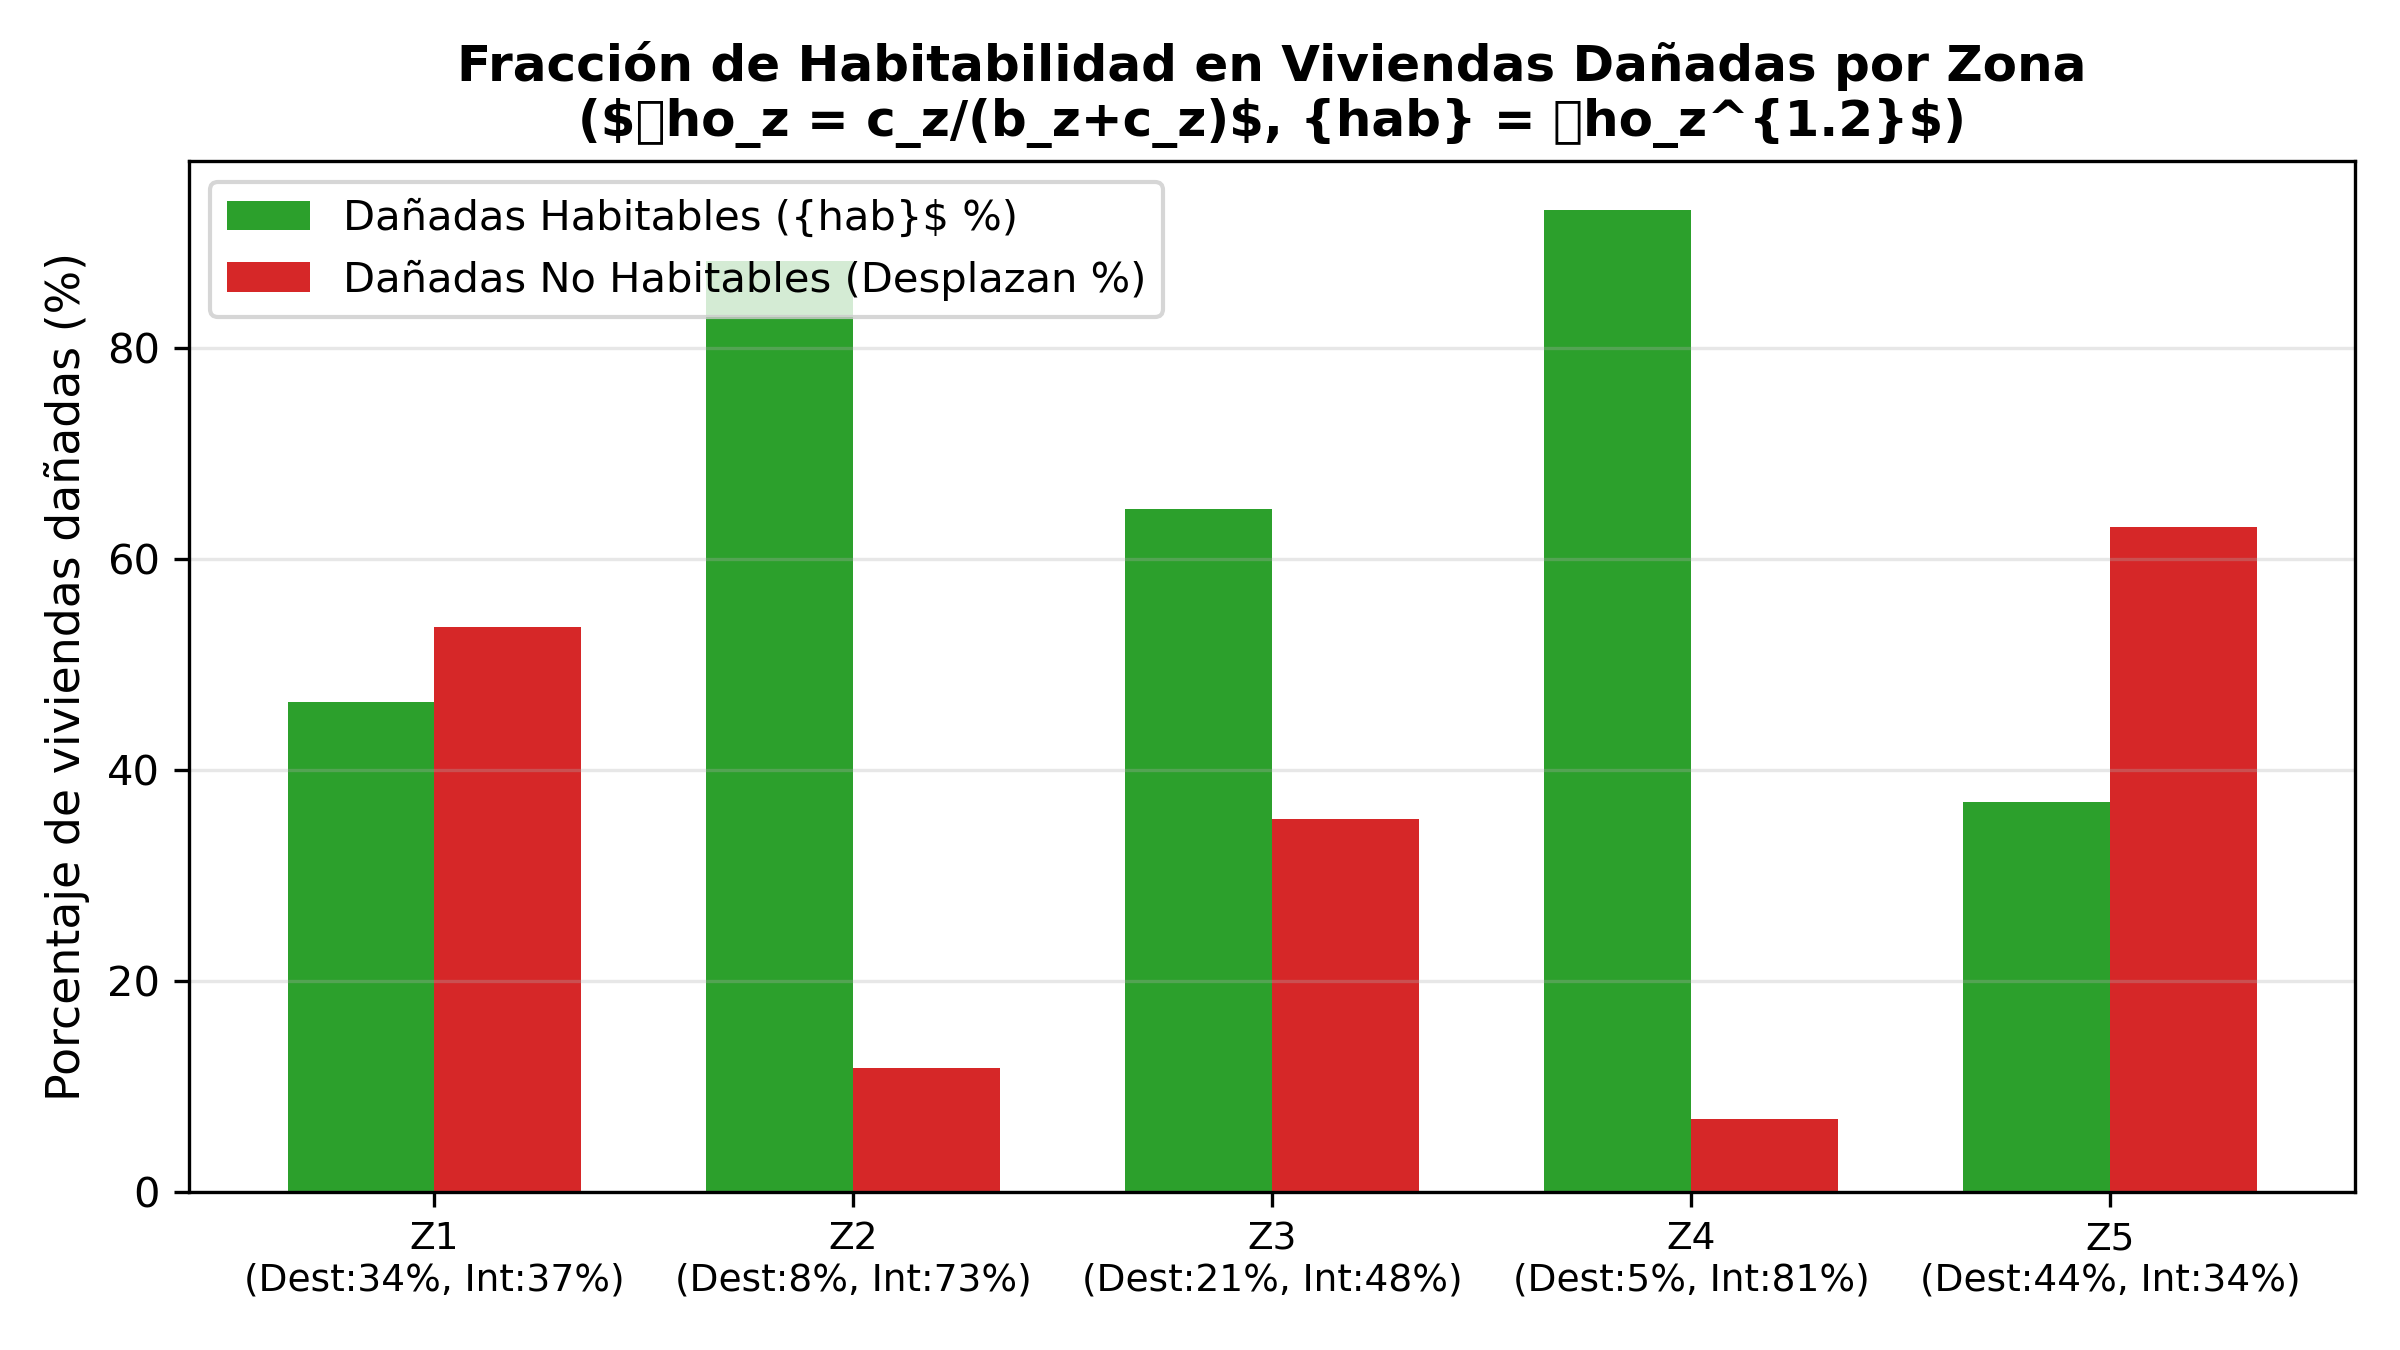
\includegraphics[width=0.68\linewidth]{grafica5_habitabilidad_viviendas.png}
    \caption{Porcentaje de viviendas dañadas habitables frente a inhabitables en cada zona.}
    \label{fig:hab}
\end{figure}

\subsection{Incertidumbre y método Monte Carlo}
Para cumplir con el requisito de reportar distribuciones y no valores aislados, implementamos una simulación Monte Carlo con 100 realizaciones independientes. En cada corrida, aplicamos un ruido estocástico normal del 10\% ($\mathcal{N}(0, 0.10)$) sobre el flujo de nuevos desplazados $N_z(t)$. A partir de estas corridas, calculamos la media y los intervalos de confianza del 95\% mediante percentiles empíricos (2.5\% y 97.5\%).

% ==============================================================================
% SECCIÓN 3: RESULTADOS Y ANÁLISIS
% ==============================================================================
\section{Resultados y análisis de la simulación}

\subsection{Comportamiento temporal y momentos críticos}
Al analizar las trayectorias de ocupación e identificar los momentos clave de la emergencia, encontramos tres patrones determinantes:

\begin{enumerate}
    \item \textbf{Saturación y colapso inmediato en cuatro zonas:} En las zonas Z1, Z2, Z3 y Z5, el sistema supera el umbral del 80\% y se llena al 100\% de su capacidad en el \textbf{Bloque 0 (las primeras 6 horas)}. La desproporción entre personas buscando refugio y la capacidad instalada es crítica. El caso más grave es Z1 (Centro histórico), donde 11,470 personas demandan refugio ante un único albergue habilitado con capacidad para solo 400 personas (una demanda 28 veces superior a la oferta). En Z5 ocurre algo similar: 14,540 damnificados llegan a instalaciones con capacidad combinada de 1,500 cupos.
    \item \textbf{La paradoja de capacidad ociosa en Z4:} La zona Z4 (Este comercial) es la \textbf{única que nunca se satura}. Inicia con un 21.7\% de ocupación y finaliza en 38.9\% (un promedio de 2,068 personas albergadas para una capacidad de 5,300 plazas). Esto significa que durante toda la emergencia existen más de 3,200 camas desocupadas en Z4, mientras en Z1 y Z5 decenas de miles de personas duermen a la intemperie.
    \item \textbf{Estabilización del sistema:} La llegada de nuevos desplazados se desacelera marcadamente entre las 36 y 48 horas (bloques T6 a T8), momento en el cual las curvas de ocupación y de personas sin alojamiento alcanzan una meseta estable.
\end{enumerate}

\begin{table}[H]
\centering
\small
\resizebox{\linewidth}{!}{%
\begin{tabular}{lcccccc}
\toprule
\textbf{Zona} & \textbf{Capacidad} & \textbf{Demanda T0} & \textbf{Ratio D/C} & \textbf{Cruce del 80\%} & \textbf{Alojados (72h) [IC 95\%]} & \textbf{Sin albergue (72h) [IC 95\%]} \\
\midrule
Z1 & 400   & 11,470 & 28.7 & Bloque 0 (0--6h) & 400 [400, 400]       & 15,198 [13,080, 17,248] \\
Z2 & 2,200 & 2,460  & 1.12 & Bloque 0 (0--6h) & 2,200 [2,200, 2,200] & 2,309 [1,740, 2,808] \\
Z3 & 2,400 & 4,510  & 1.88 & Bloque 0 (0--6h) & 2,400 [2,400, 2,400] & 4,857 [3,913, 5,753] \\
Z4 & 5,300 & 1,150  & 0.22 & \textbf{Nunca} (máx 38.9\%) & 2,068 [1,806, 2,297] & \textbf{0 [0, 0]} \\
Z5 & 1,500 & 14,540 & 9.69 & Bloque 0 (0--6h) & 1,500 [1,500, 1,500] & 19,884 [16,931, 22,779] \\
\midrule
\textbf{Total} & \textbf{11,800} & \textbf{34,130} & \textbf{2.89} & \textbf{Bloque 0 (0--6h)} & \textbf{8,568 [8,306, 8,797]} & \textbf{42,248 [35,664, 48,588]} \\
\bottomrule
\end{tabular}%
}
\end{table}

\begin{figure}[H]
    \centering
    \begin{minipage}{0.49\linewidth}
        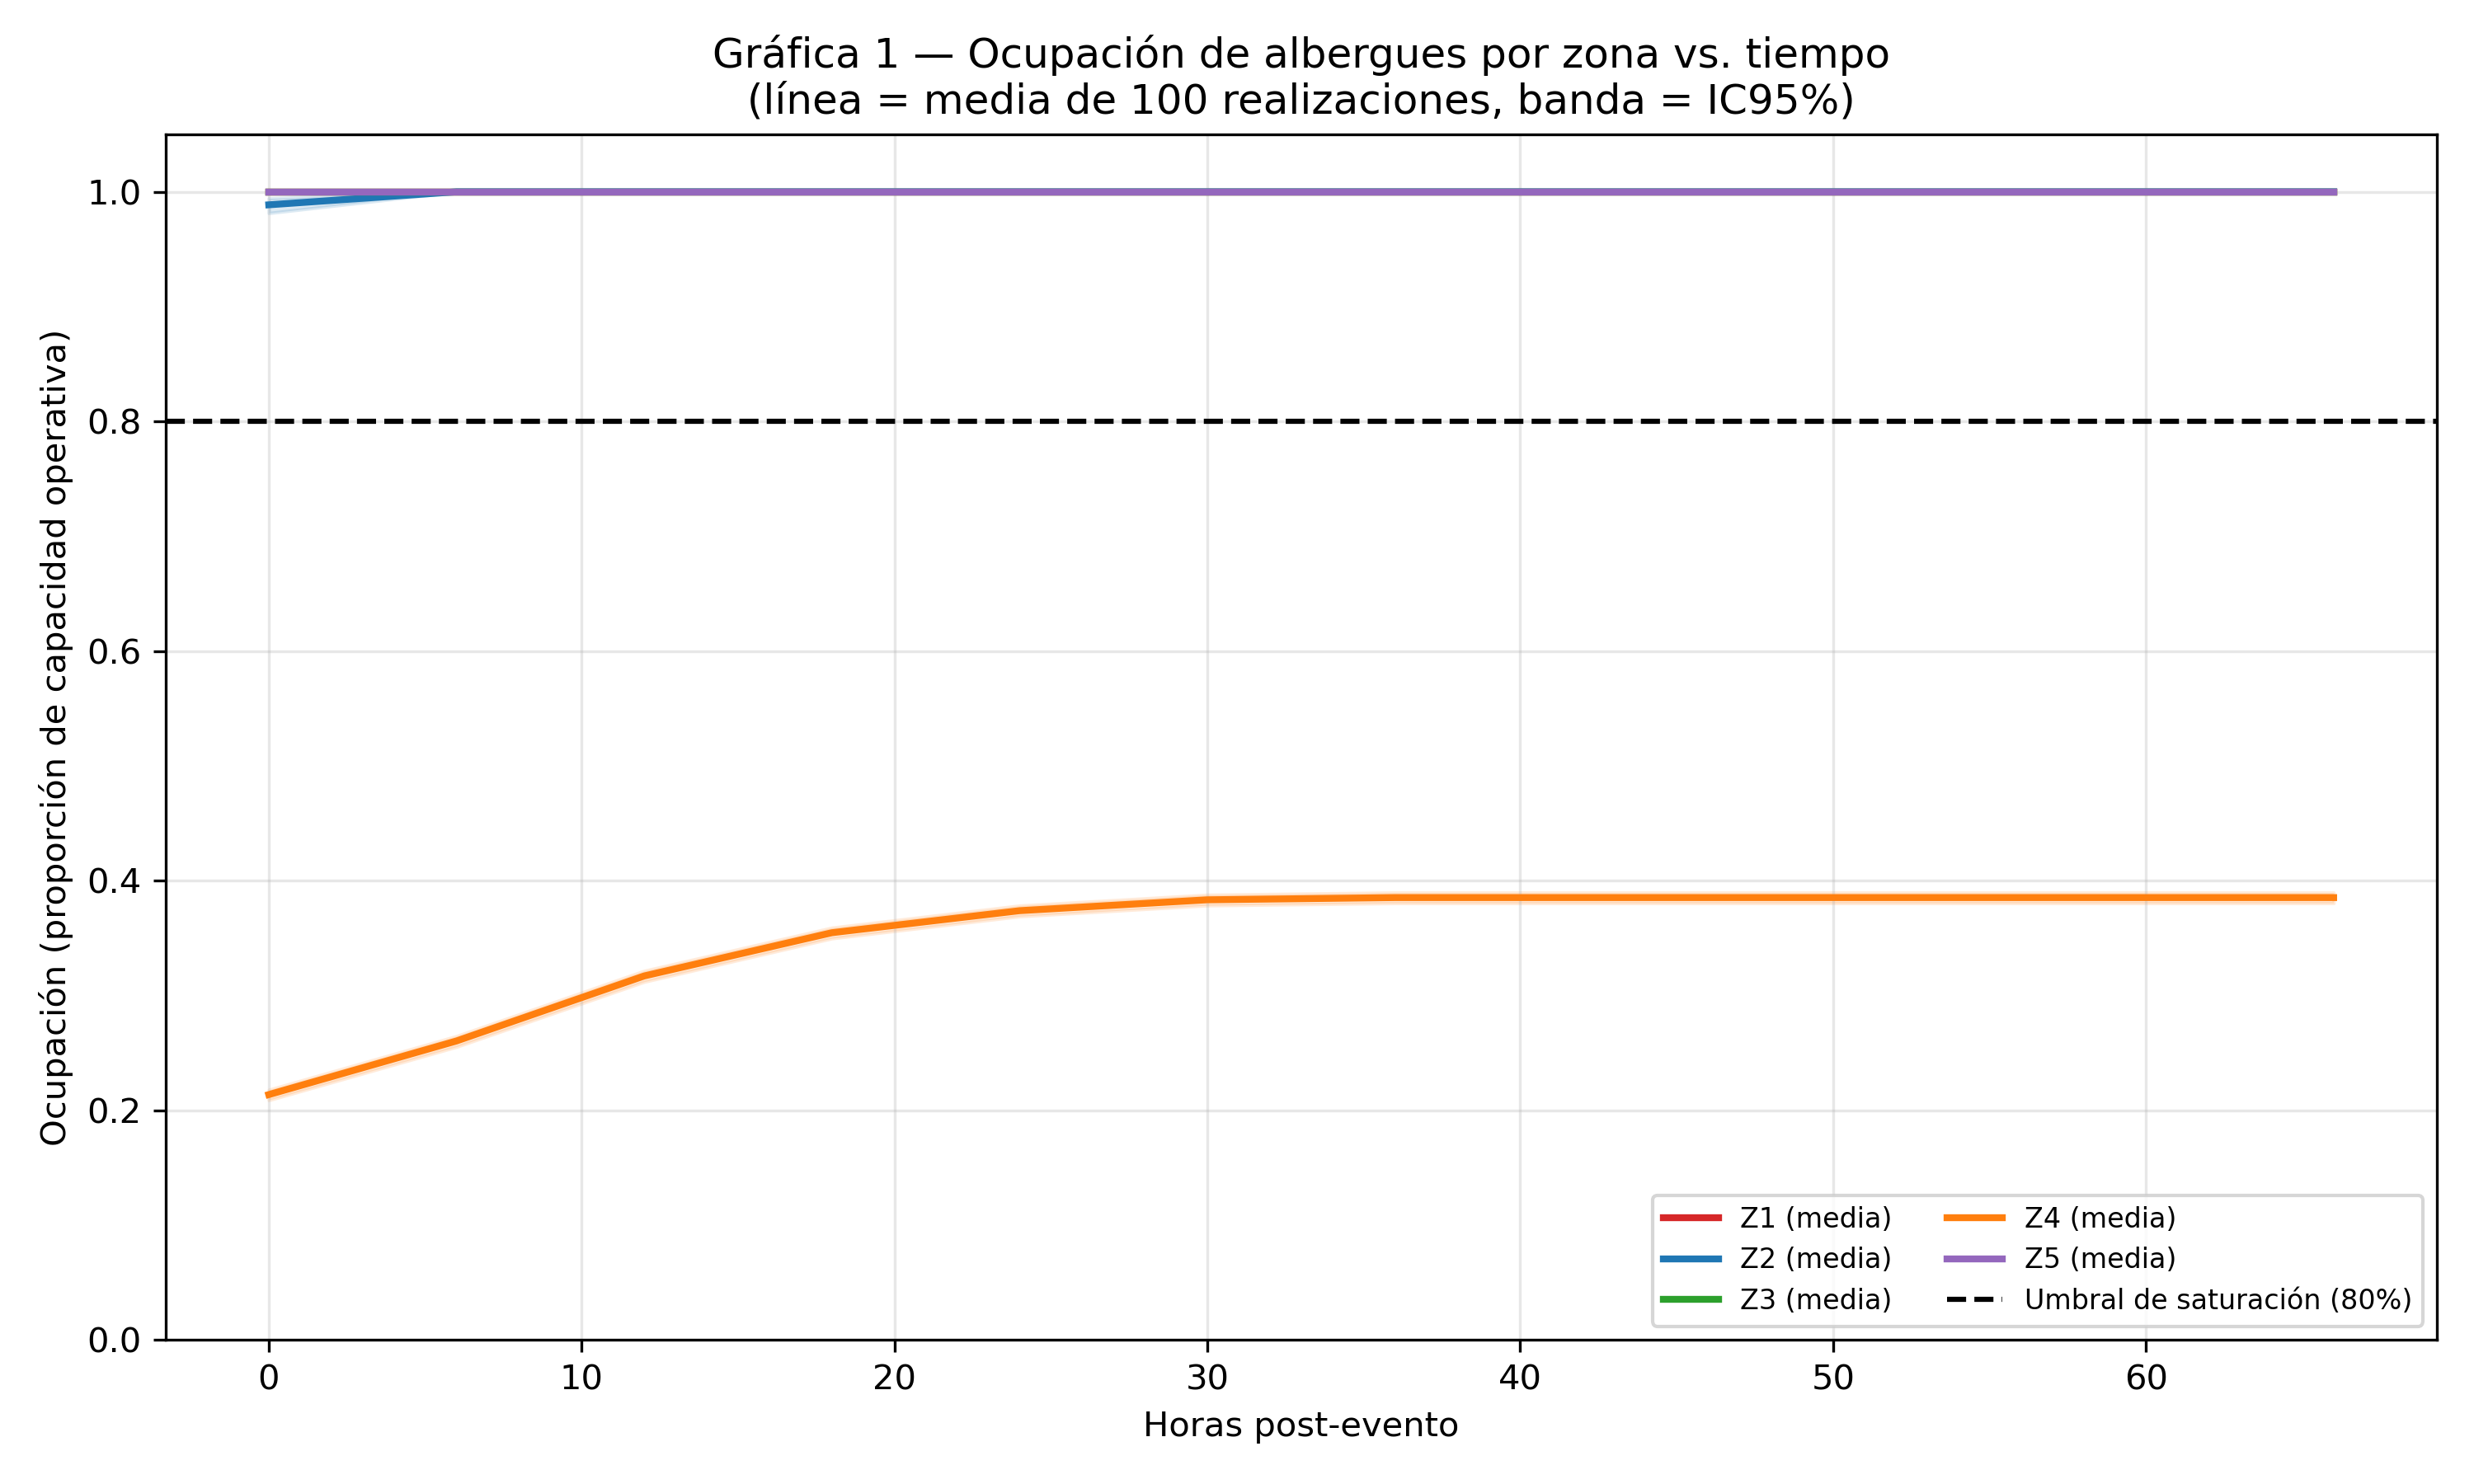
\includegraphics[width=\linewidth]{grafica1_ocupacion.png}
        \caption{Ocupación de albergues frente al umbral del 80\%.}
        \label{fig:ocupacion}
    \end{minipage}\hfill
    \begin{minipage}{0.49\linewidth}
        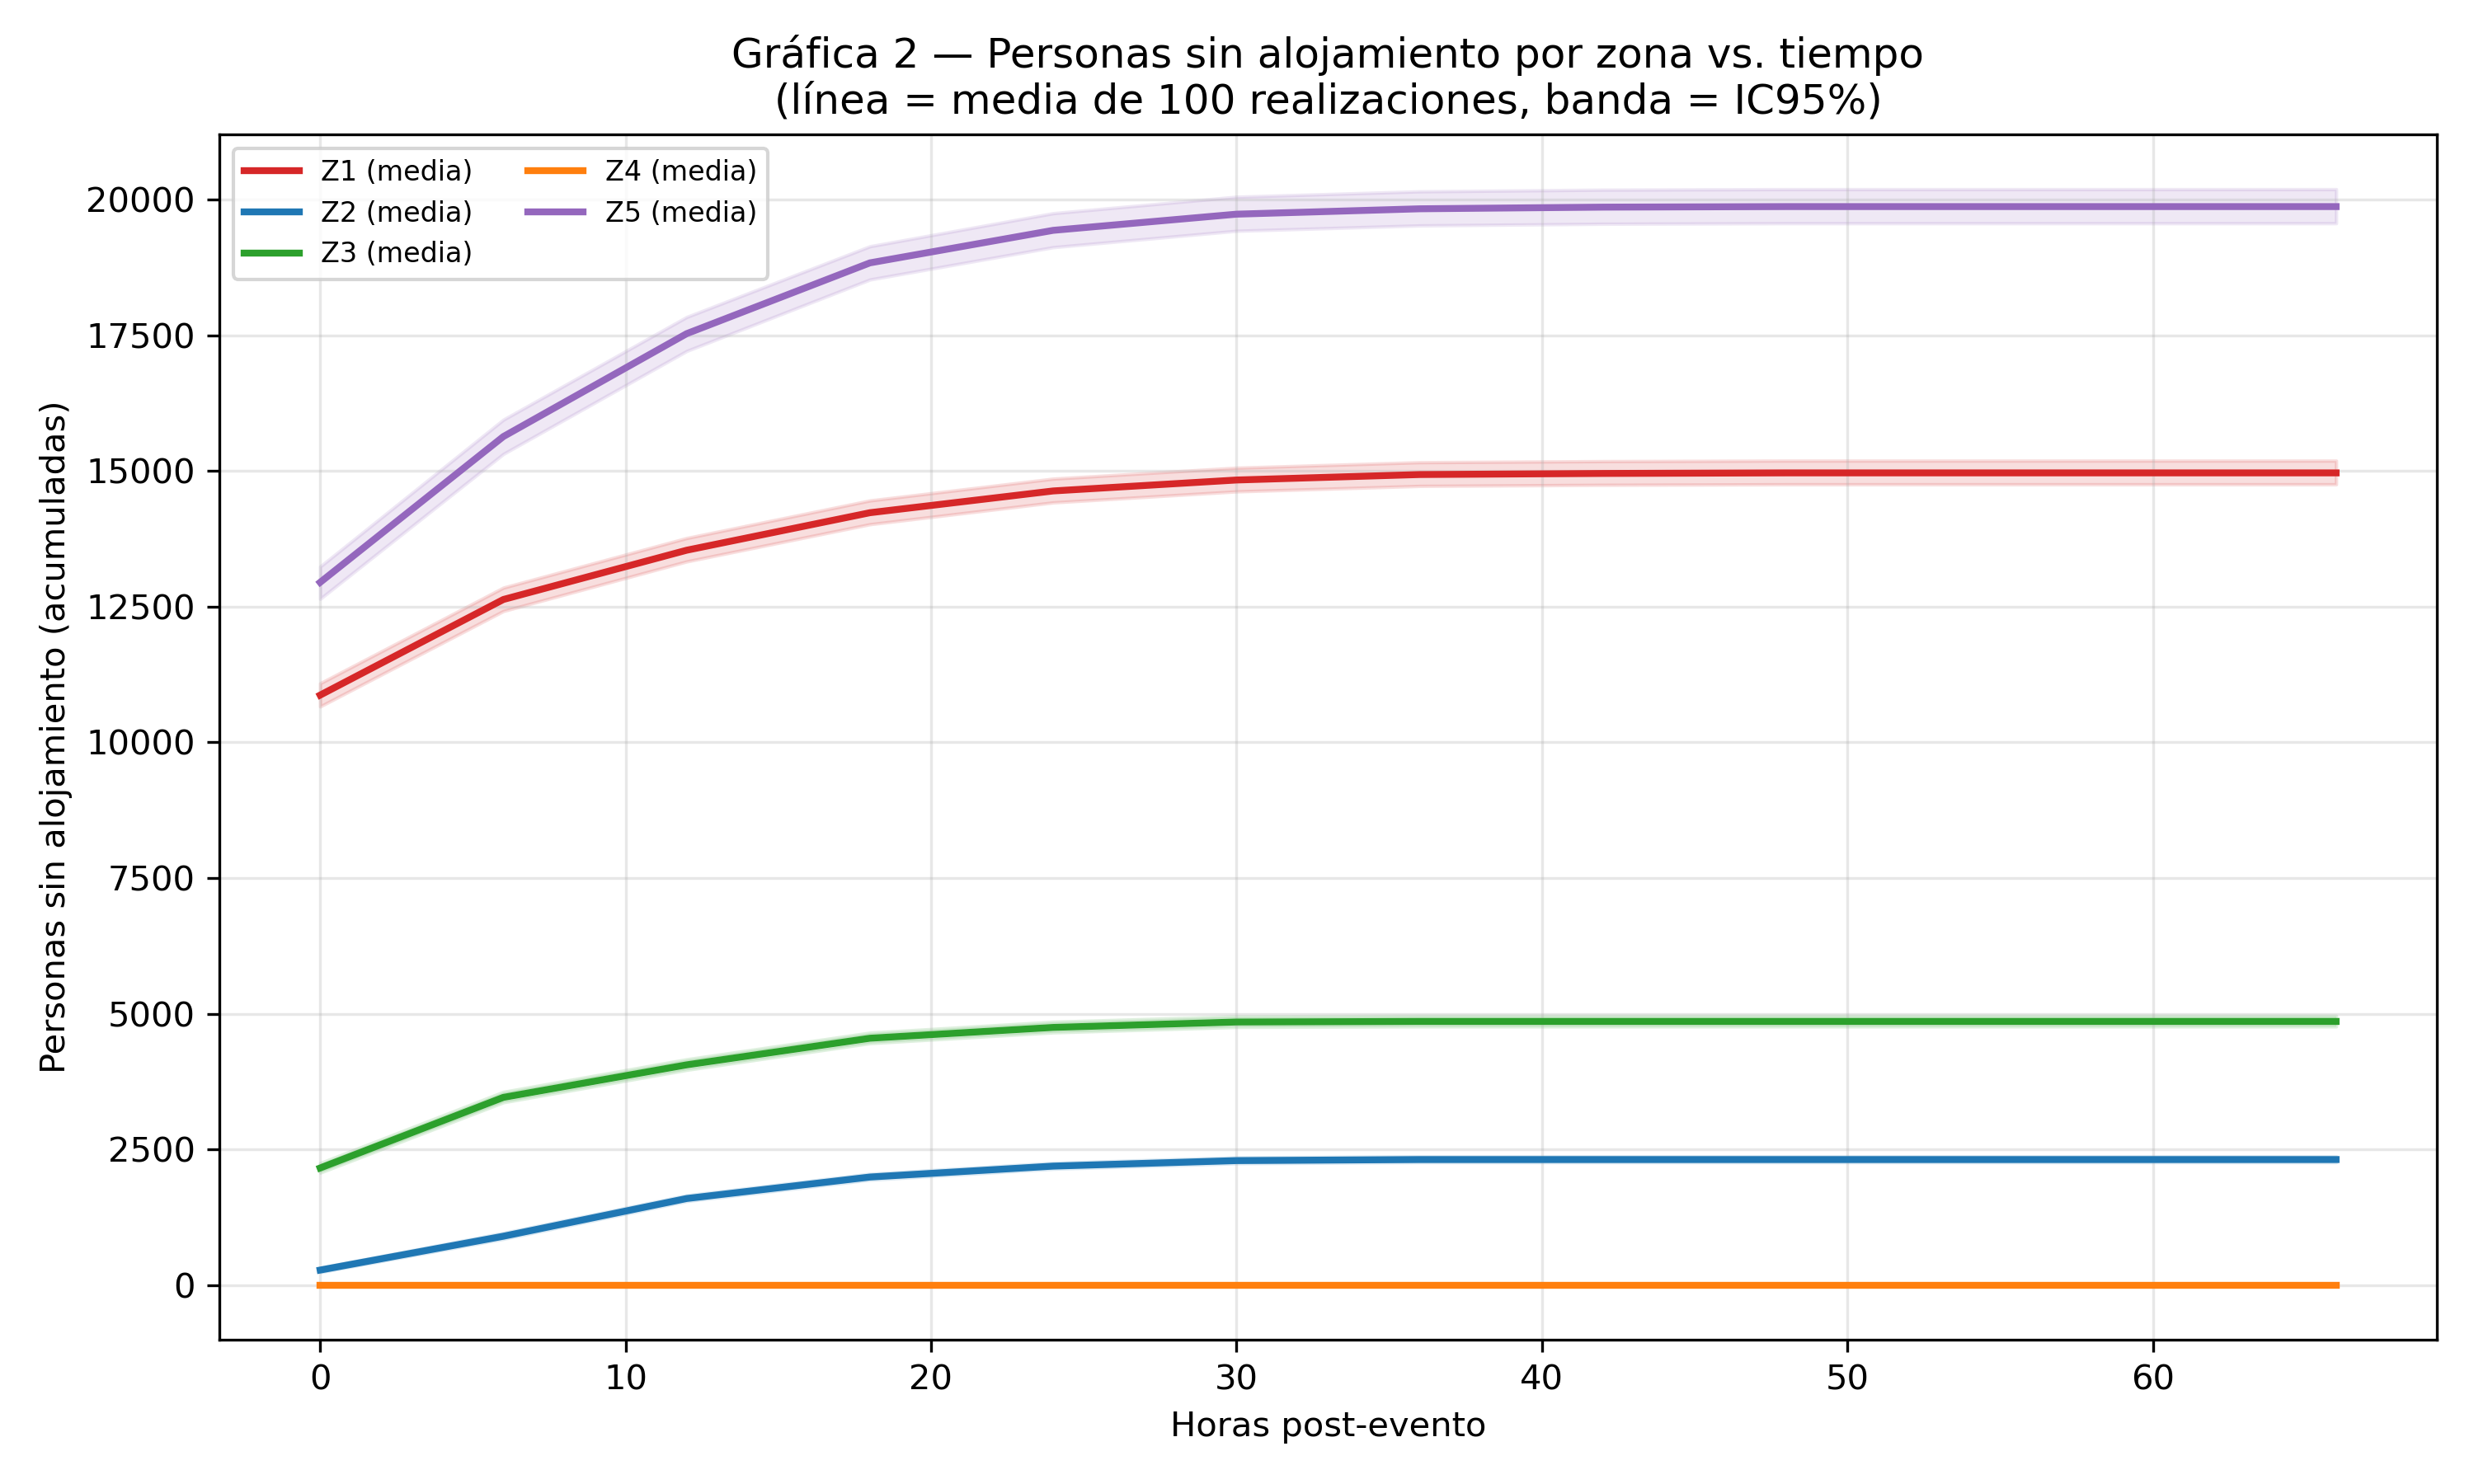
\includegraphics[width=\linewidth]{grafica2_sin_alojamiento.png}
        \caption{Personas sin albergue en la vía pública.}
        \label{fig:no_alojados}
    \end{minipage}
\end{figure}

\subsection{Respuesta a la Pregunta 1 del examen (Análisis propio)}
\textbf{¿En qué zona y bloque de tiempo el sistema supera el 80\% de capacidad por primera vez?}
El sistema supera el umbral del 80\% de manera inmediata en el \textbf{Bloque 0 (primeras 6 horas)} en cuatro de las cinco zonas simultáneamente: \textbf{Z1, Z2, Z3 y Z5}. La única zona que se mantiene por debajo es Z4.

\textbf{¿Qué ocurre con las personas que no encuentran lugar y cómo afecta la dinámica en los bloques siguientes?}
En las primeras 6 horas, más de 25,000 personas no consiguen espacio en los albergues habilitados, cifra que crece hasta alcanzar las 42,248 personas a las 72 horas. Dado que el modelo base no contempla traslados hacia Z4 ni ampliación de albergues, estas personas quedan en la calle o en campamentos improvisados. Esto provoca tres consecuencias graves:
\begin{itemize}
    \item \textbf{Aumento del riesgo de salud:} La permanencia a la intemperie eleva las enfermedades respiratorias e infecciones, por lo que la necesidad médica real tenderá a superar la tasa nominal del 18\% calculada inicialmente.
    \item \textbf{Desabastecimiento humanitario:} Como la entrega de suministros (Grupo 3) se calcula exclusivamente para las personas dentro de los albergues oficiales ($1.00 \times A_z(t)$), las más de 42,000 personas fuera de ellos quedan formalmente desatendidas en el plan logístico inicial.
    \item \textbf{Presión sobre otras zonas:} Esta masa de población sin techo genera tensiones sociales y presiona por migrar hacia zonas con mejores servicios como Z4.
\end{itemize}

\subsection{Entregas a los Grupos 2 y 3}
\begin{itemize}
    \item \textbf{Demanda médica para Grupo 2 (18\% de desplazados):} Al final de las 72 horas, la ciudad acumula una demanda esperada de \textbf{9,147 atenciones médicas} (IC 95\%: [7,908; 10,362]). La mayor parte se concentra en Z5 (3,849 pacientes) y Z1 (2,808 pacientes), señalando con claridad dónde deben reforzarse los hospitales de campaña.
    \item \textbf{Demanda de víveres para Grupo 3 (100\% de albergados):} Debido a que los albergues de cuatro zonas se llenan desde el inicio, la demanda de raciones se congela rápidamente en \textbf{8,568 raciones por bloque de 6h} a nivel ciudad, de las cuales 2,068 corresponden a Z4, 2,400 a Z3, 2,200 a Z2, 1,500 a Z5 y apenas 400 a Z1.
\end{itemize}

% ==============================================================================
% SECCIÓN 4: INCORPORACIÓN DEL INTERCAMBIO PRESENCIAL
% ==============================================================================
\section{Incorporación del intercambio de información}

\subsection{Intercambio con Grupo 6 y respuesta a la Pregunta 2}
Durante el intercambio presencial, recibimos de parte del Grupo 6 la proyección del flujo de evacuación calculada a partir de su modelo de comportamiento poblacional. 

\textbf{¿Qué supuesto de nuestro modelo inicial era incorrecto y cómo se corrigió?}
El supuesto inicial que resultó incorrecto fue asumir que las personas desplazadas llegaban de golpe a los albergues desde el primer instante (T0), siguiendo la curva estática de los datos preliminares. El Grupo 6 nos explicó que esto no ocurre así en la realidad por dos factores principales:
\begin{enumerate}
    \item En las zonas más dañadas (Z1 y Z5), entre el 35\% y el 50\% de las personas afectadas no pueden salir por sus propios medios en las primeras 12 horas debido a escombros en las calles, lesiones o familiares atrapados, dependiendo de la ayuda de rescatistas (coordinados por Grupo 5).
    \item La confusión inicial, las noticias falsas y el temor a que saqueen sus hogares hacen que muchas familias decidan quedarse cerca de sus viviendas durante las primeras horas en lugar de dirigirse de inmediato a un albergue.
\end{enumerate}
Para corregirlo, adaptamos nuestro flujo de entrada $N_z(t)$: redujimos la llegada masiva en T0 y T1 y trasladamos ese contingente hacia los bloques T2 (12--18h) y T3 (18--24h), momento en que las cuadrillas de rescate logran habilitar vías y evacuar a la población retenida.

\begin{figure}[H]
    \centering
    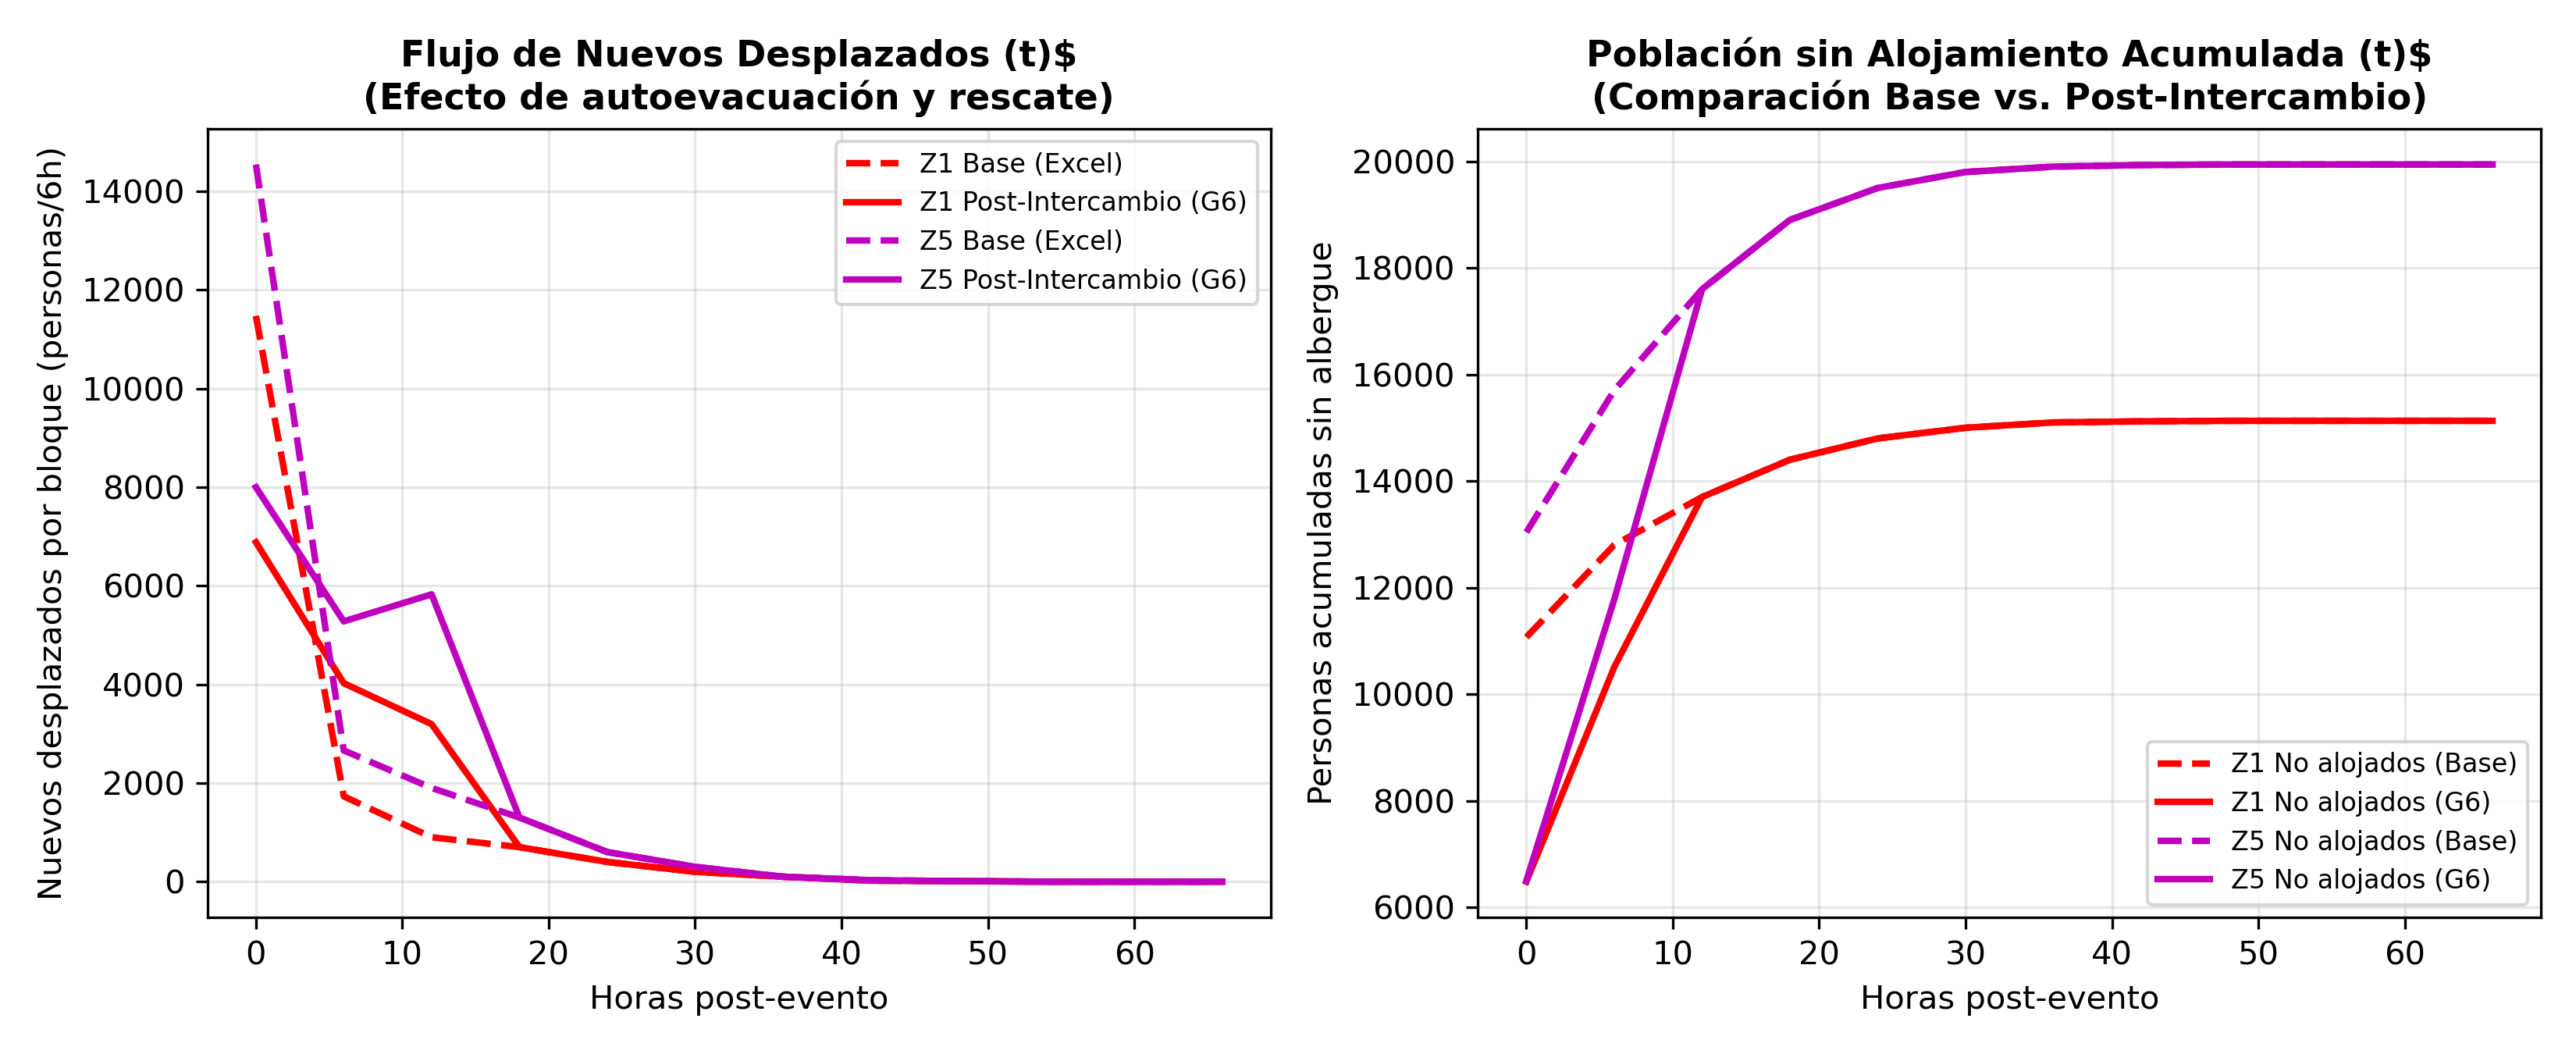
\includegraphics[width=0.85\linewidth]{grafica6_comparativa_intercambio.png}
    \caption{Comparación de la llegada de desplazados y acumulación de personas sin albergue antes y después de incorporar la información del Grupo 6.}
    \label{fig:intercambio}
\end{figure}

\textbf{¿En cuántas horas difiere el momento de colapso de los albergues entre ambas estimaciones?}
\begin{itemize}
    \item En \textbf{Z1 y Z5}, el momento en que se supera el 80\% \textbf{no cambia (difiere en 0 horas)}. La capacidad de estos albergues es tan pequeña frente al tamaño de la población damnificada que, aun reteniendo a la mitad de la gente en sus casas durante las primeras 12 horas, la cantidad de personas que llega en T0 sigue superando con creces los 400 cupos de Z1 y los 1,500 de Z5.
    \item No obstante, la gran diferencia radica en el \textbf{colapso del espacio público exterior}: el pico masivo de personas desbordando las calles alrededor de los albergues no ocurre al amanecer, sino que \textbf{se retrasa 12 horas} (se traslada a la ventana de 12 a 18 horas).
    \item En \textbf{Z3}, donde la relación demanda/capacidad es más ajustada, el colapso del albergue se retrasa en \textbf{6 horas} (pasa de T0 a T1), abriendo una ventana de oportunidad invaluable para habilitar instalaciones adicionales.
\end{itemize}

% ==============================================================================
% SECCIÓN 5: LIMITACIONES Y PROPUESTAS DE MEJORA
% ==============================================================================
\section{Limitaciones del modelo y propuestas de mejora}

\subsection{Limitación 1: Aislamiento estricto entre zonas}
El modelo asume que cada zona opera de forma completamente aislada ($\text{Reubicados}_z = 0$). Este supuesto genera una situación poco realista: mientras en Z1 y Z5 hay más de 35,000 personas en la calle, en Z4 hay más de 3,200 camas desocupadas que nadie utiliza. En una emergencia real, las familias se desplazan a zonas vecinas o las autoridades organizan transporte en autobuses.

\textbf{Propuesta de mejora:} Incorporar una tasa de reubicación interzonal que traslade personas sin alojamiento de las zonas saturadas hacia los albergues con cupos libres, condicionada a la accesibilidad de las calles que reporta el Grupo 4.

\subsection{Limitación 2: Capacidad fija de albergues en el tiempo}
El modelo asume que la capacidad de los albergues no cambia durante las 72 horas. Esto no refleja los esfuerzos de respuesta que se realizan en el terreno, donde cuadrillas municipales y voluntarios habilitan galpones, instalan carpas o reparan escuelas dañadas.

\textbf{Propuesta de mejora:} Conectar la capacidad de los albergues con el cronograma de reparaciones del Grupo 4 y la asignación de personal del Grupo 5, de modo que la capacidad crezca dinámicamente conforme se despliegan recursos técnicos.

\subsection{Respuesta a la pregunta abierta para el video (Punto 4)}
\textit{«Su modelo proyecta el flujo de desplazados hacia los albergues, pero los albergues no son el único destino posible: algunas personas se quedan con familiares, otras permanecen en sus viviendas dañadas por miedo o desinformación. ¿Qué supuesto de su modelo considera que tiene mayor potencial de invalidar sus conclusiones sobre el colapso del sistema de albergues, y qué datos reales necesitaría para corregirlo?»}

\textbf{Respuesta del Grupo 1:}
El supuesto que tiene mayor potencial de invalidar (o sobreestimar) la velocidad de colapso de los albergues es \textbf{asumir que toda persona con vivienda afectada busca refugio en un albergue público}. 

En Guatemala y en desastres similares en la región, la primera red de respuesta ante un terremoto no son las instituciones del Estado, sino la solidaridad comunitaria y familiar. Entre el 40\% y el 60\% de las personas que no pueden dormir en sus casas suelen alojarse con familiares o amigos que viven en zonas menos afectadas (como Z2 o Z4). Además, muchas familias deciden levantar carpas precarias en la banqueta frente a su casa para evitar saqueos de sus pertenencias. Al no considerar estas alternativas, nuestro modelo asume que toda la demanda presiona directamente sobre las instalaciones municipales.

Para corregir este supuesto en una emergencia real, necesitaríamos dos fuentes de datos:
\begin{enumerate}
    \item Los resultados preliminares de la ficha de Evaluación de Daños y Análisis de Necesidades (EDAN de CONRED) levantada en las primeras horas, que consulta a las familias si cuentan con red de apoyo familiar.
    \item Datos agregados y anonimizados de movilidad por antenas de telefonía móvil, que permitirían verificar qué porcentaje de damnificados se trasladó a casas particulares fuera del área de impacto.
\end{enumerate}
Incorporar este factor reduciría la demanda directa sobre albergues en aproximadamente un 50\%, lo que aliviaría la saturación en Z2 y Z3 y permitiría que el gobierno municipal concentre todos sus recursos logísticos en las zonas verdaderamente críticas: Z1 y Z5.

\end{document}
